%--------------------------------------------------
\subsection{Prototipo 2: Integración con Apache Kafka}

El prototipo 2 de la aplicación incluye las modificaciones en el diseño inicial de la aplicación para mostrar a los clientes que se hayan conectado a un Beacon que pertenece al departamento actual donde se encuentra el vendedor y la integración de la aplicación con los servicios REST para obtener la información de los mismos. De igual forma dentro de este prototipo se incluye el diseño para que el vendedor edite sus datos de perfil y su respectiva integración con el servidor para hacer la persistencia de los datos. \\ \par

%--------------------------------------------------
\subsubsection{Análisis}

Dentro del análisis para el desarrollo de este prototipo se incorporan los requerimientos funcionales \hyperlink{RFAPV}{RFAPV3 Editar perfil del vendedor} y \hyperlink{RFAPV}{RFAPV2 Visualizar clientes cercanos}, definidos previamente en el capítulo del ``Bosquejo general de la aplicación''  con el título de ``Requerimientos funcionales de la Aplicación Interactiva para el Personal de Ventas''. \\ \par

\paragraph{Casos de uso de la AIPV.} ~\\

La figura \ref{casos-uso-AIPV1} definida previamente en el prototipo 1, muestra los casos de uso de la AIPV.

\paragraph{Diagrama de clases.} ~\\

La figura \ref{clases-AIPV2} presenta el diagrama de clases para el prototipo 2 de la AIPV. Para una mejor visualización, el diagrama se ha dividido en 3 partes. 

\FloatBarrier
\begin{figure}[htbp!]
		\centering
			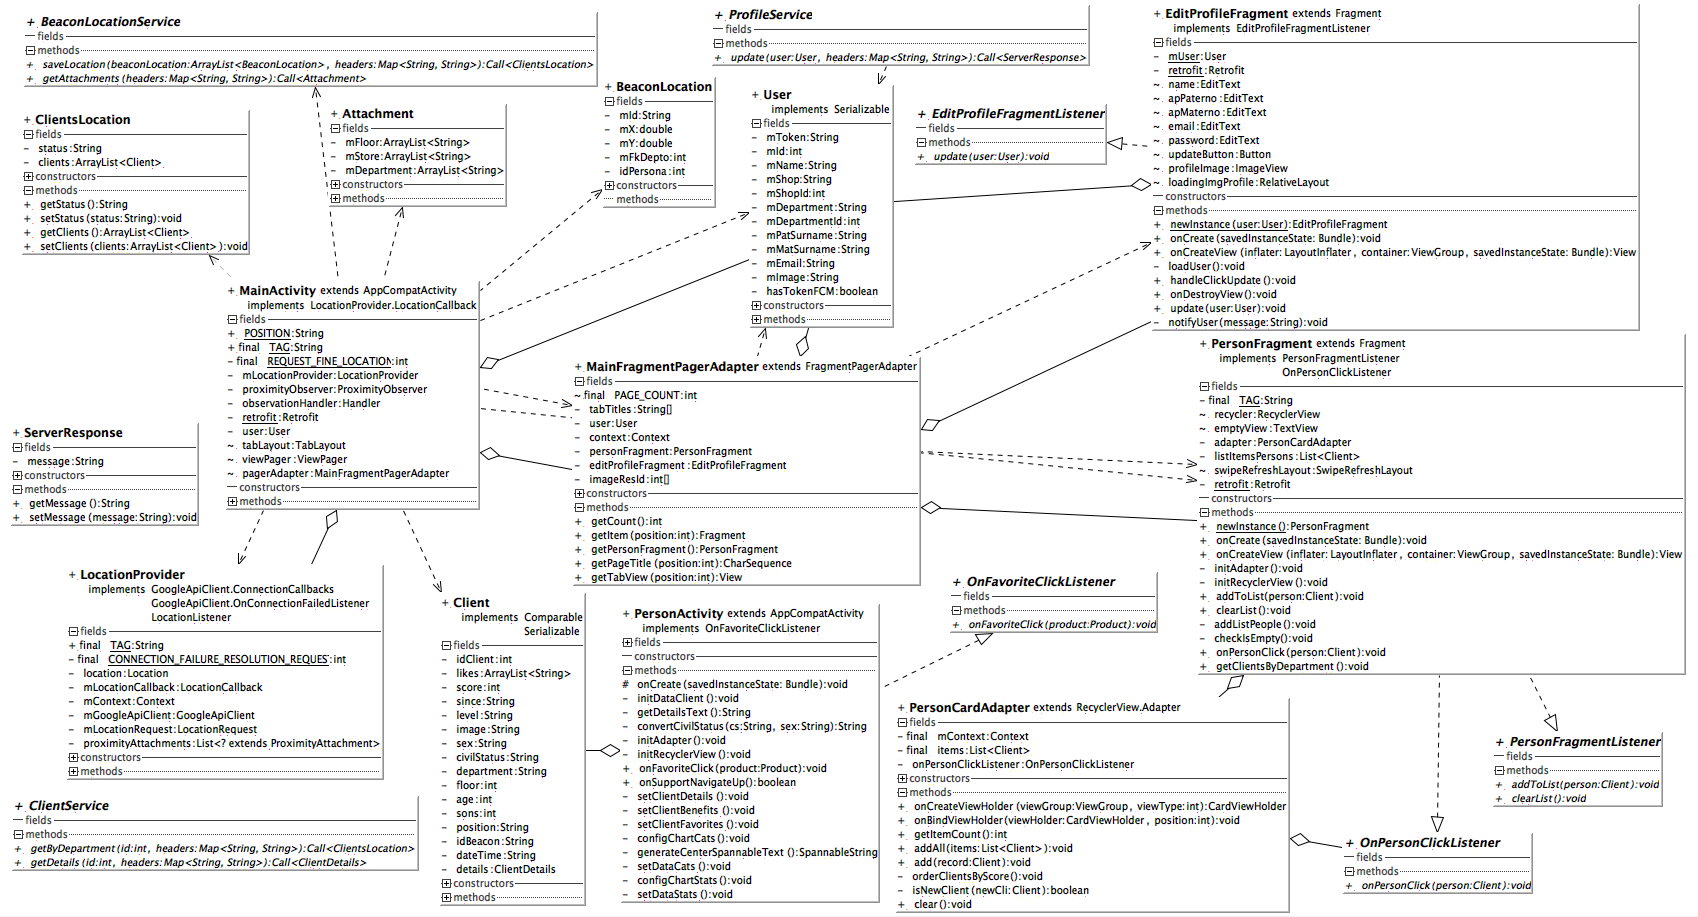
\includegraphics[width=.9 \textwidth]{imagenes/adrian/vendedor/prototipo2/clases}
		\caption{Diagrama de clases del prototipo 2 de la AIPV (Visualización completa).}
		\label{clases-AIPV2}
\end{figure}
\FloatBarrier

La descripción de los nuevos elementos de la figura \ref{clases-AIPV2-parte1} es la siguiente: 

\begin{itemize}
\item \textbf{ClientsLocation}: Clase que retrofit mapea para la respuesta de la API REST al enviar la ubicación de un Beacon la cual contiene un estatus y un arreglo de Clientes que son los cercanos al Beacon.
\item \textbf{ServerResponse}: Clase que retrofit mapea para la respuesta de algunos endpoints de la API REST, por ejemplo al actualizar la información de perfil de un vendedor. La clase contiene un mensaje que el servidor envía para notificar los cambios realizados.
\item \textbf{Client}: Clase con la información necesaria de un cliente cercano. 
\item \textbf{ClientService}: Interfaz que define dos métodos GET , el primero getByDepartment, para obtener a los clientes más recientes cercanos a un departamento por su id; getDetails para obtener más detalles sobre un cliente en especifico mediante su id de persona.
\end{itemize}

\FloatBarrier
\begin{figure}[htbp!]
		\centering
			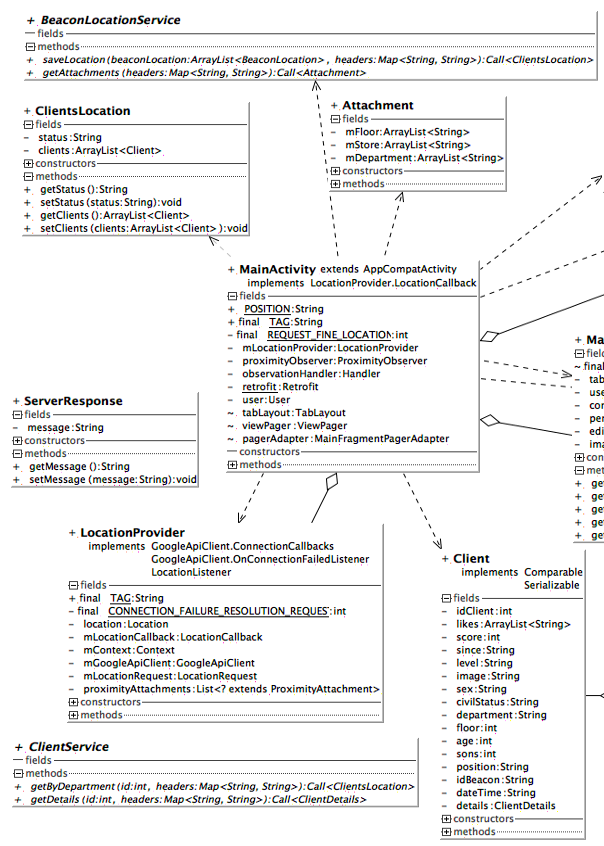
\includegraphics[width=.9 \textwidth]{imagenes/adrian/vendedor/prototipo2/clases_1}
		\caption{Diagrama de clases del prototipo 2 de la AIPV (Parte 1) .}
		\label{clases-AIPV2-parte1}
\end{figure}
\FloatBarrier

La descripción de los nuevos elementos de la figura \ref{clases-AIPV2-parte2} es la siguiente: 

\begin{itemize}
\item \textbf{ProfileService}: Interfaz que define el método update de tipo PUT, que permite enviar la información del perfil del vendedor para ser actualizada, recibe como respuesta la clase ServerResponse.
\item \textbf{EditProfileFragmentListener}: Interfaz que define el método update, la interfaz se implementa en la clase EditProfileFragment y sirve para enviar la información del perfil del vendedor para ser actualizada.
\item \textbf{MainFragmentPagerAdapter}: Clase que extiende de FragmentPagerAdapter y nos permite crear un paginador de fragmentos los cuales incluye a PersonFragment y EditProfileFragment, en esta clase se crean nuevas instancias de las mismas para organizarlas en forma de pestañas.
\item \textbf{PersonActivity}: Clase que extiende de AppCompatActivity y en la que se muestra exclusivamente los datos de un cliente.
\item \textbf{PersonCardAdapter}: Clase que extiende de RecyclerView.Adapter y funciona como el adaptador del arreglo de clientes que se muestran en un CardView, esto nos permite ocupar una sola vista para todos los clientes y ordenarlos horizontalmente en forma de lista.

\end{itemize}

\FloatBarrier
\begin{figure}[htbp!]
		\centering
			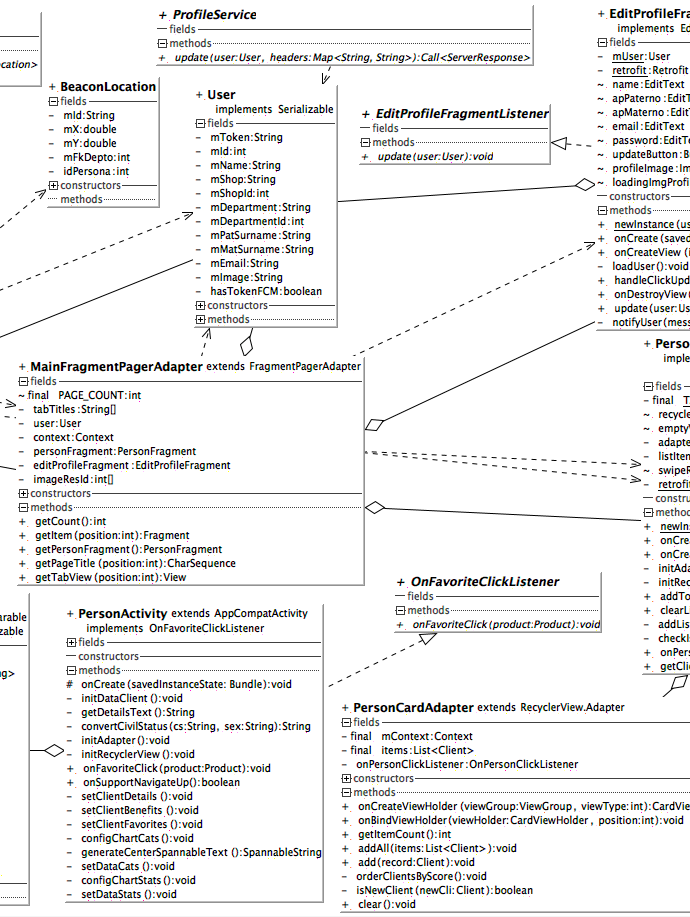
\includegraphics[width=.9 \textwidth]{imagenes/adrian/vendedor/prototipo2/clases_2}
		\caption{Diagrama de clases del prototipo 2 de la AIPV (Parte 2) .}
		\label{clases-AIPV2-parte2}
\end{figure}
\FloatBarrier

La descripción de los nuevos elementos de la figura \ref{clases-AIPV2-parte3} es la siguiente: 

\begin{itemize}
\item \textbf{PersonFragmentListener}: Interfaz que define los métodos addToList y clearList, la interfaz se implementa en la clase PersonFragment, los métodos sirven para agregar y eliminar datos de la lista de los clientes que se muestran en el fragmento.
\item \textbf{OnPersonClickListener}: Interfaz que define el método onPersonClick, la interfaz se implementa en la clase PersonFragment y sirve para iniciar la actividad PersonActivity desde el fragmento PersonFragment.
\item \textbf{EditProfileFragment}: Clase que extiende de Fragment e implementa la clase EditProfileFragmentListener, es el fragmento en el que se muestra el formulario para actualizar los datos del perfil del cliente.
\item \textbf{PersonFragment}: Clase que extiende de Fragment e implementa las clases PersonFragmentListener y OnPersonClickListener, es el fragmento en el que se muestra la lista de los clientes cercanos.
\end{itemize}

\FloatBarrier
\begin{figure}[htbp!]
		\centering
			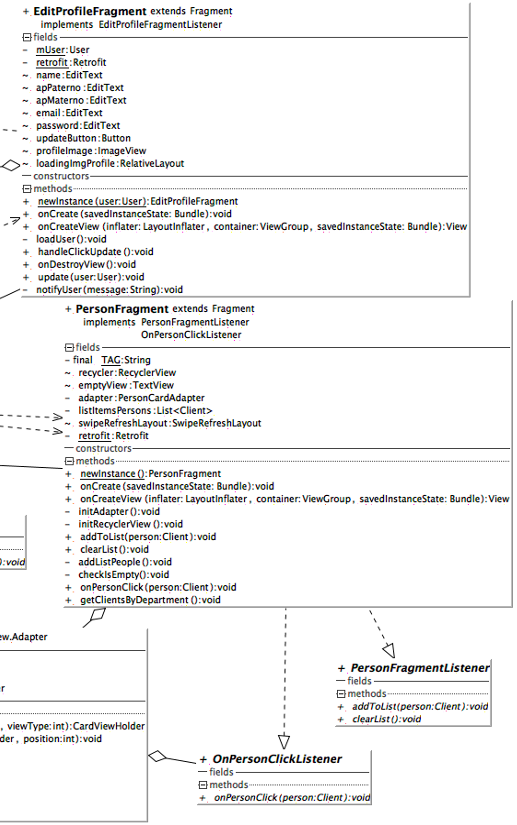
\includegraphics[width=.8 \textwidth]{imagenes/adrian/vendedor/prototipo2/clases_3}
		\caption{Diagrama de clases del prototipo 2 de la AIPV (Parte 3) .}
		\label{clases-AIPV2-parte3}
\end{figure}
\FloatBarrier


%--------------------------------------------------
\subsubsection{Diseño}

A partir de los requerimientos definidos para este prototipo se muestran los casos de uso y diagramas de secuencia.\\ \par


\paragraph{Diagramas de secuencia.} ~\\

\title{\textbf{Obtener estadísticas del cliente.}\\}

En la figura \ref{secuencia-AIPV2-perfil} se muestra el diagrama de secuencia para editar perfil en la AIPV, el cual describe los pasos que se llevan  a cabo para que el usuario vendedor edite sus datos de perfil correctamente. Para una mejor visualización el diagrama se ha dividido en 2 partes las cuales se muestran en las figuras \ref{secuencia-AIPV2-perfilUno} y \ref{secuencia-AIPV2-perfilDos} .

\FloatBarrier
\begin{figure}[htbp!]
		\centering
			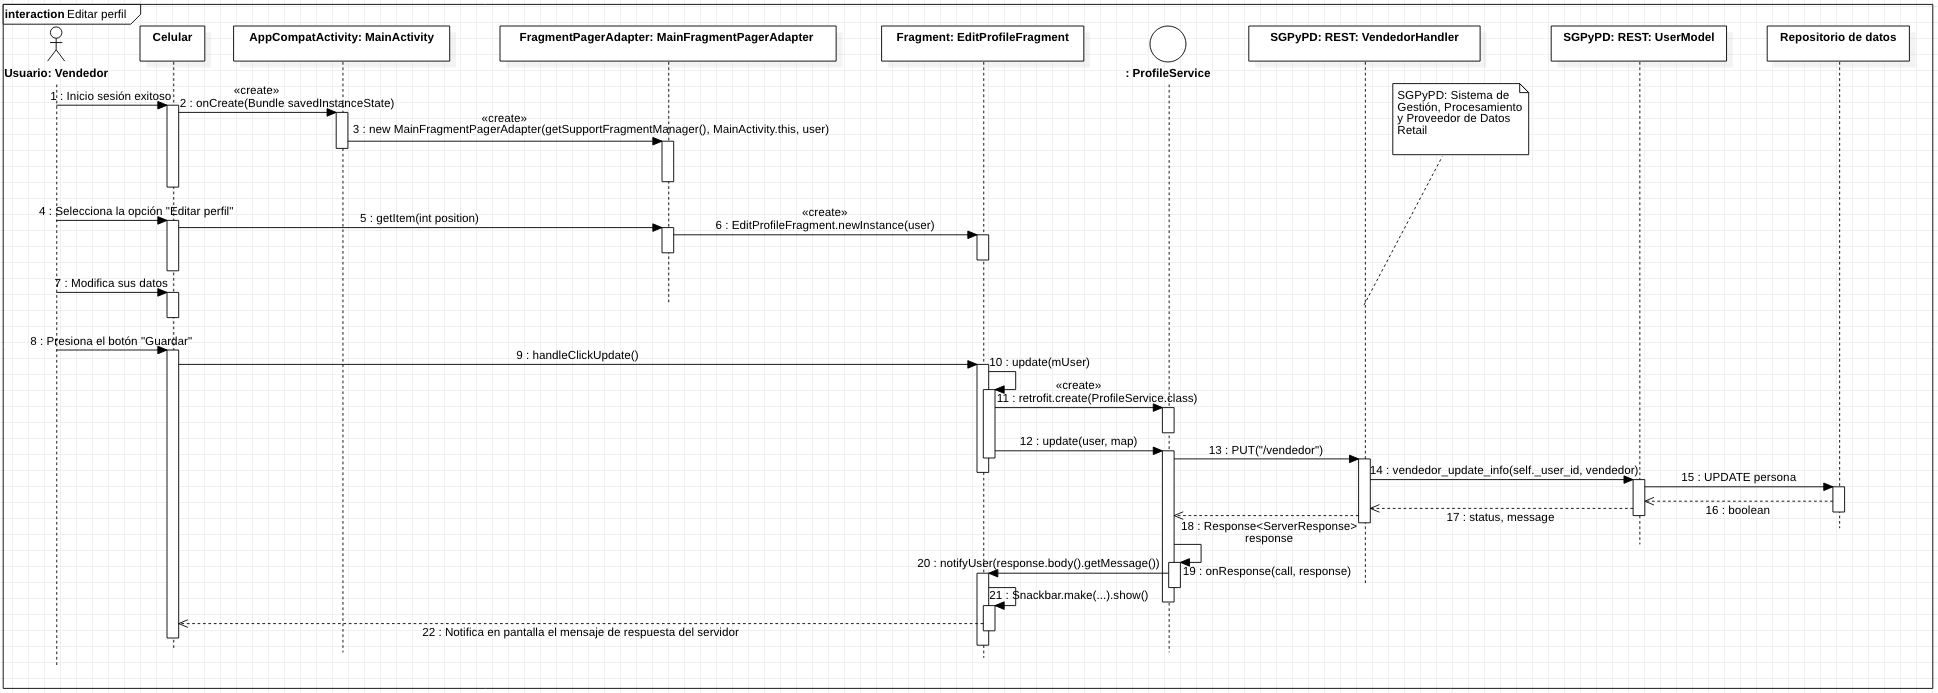
\includegraphics[width=1 \textwidth]{imagenes/adrian/vendedor/prototipo2/editar_perfil}
		\caption{Diagrama de secuencia para editar perfil de un vendedor.}
		\label{secuencia-AIPV2-perfil}
\end{figure}
\FloatBarrier

\FloatBarrier
\begin{figure}[htbp!]
		\centering
			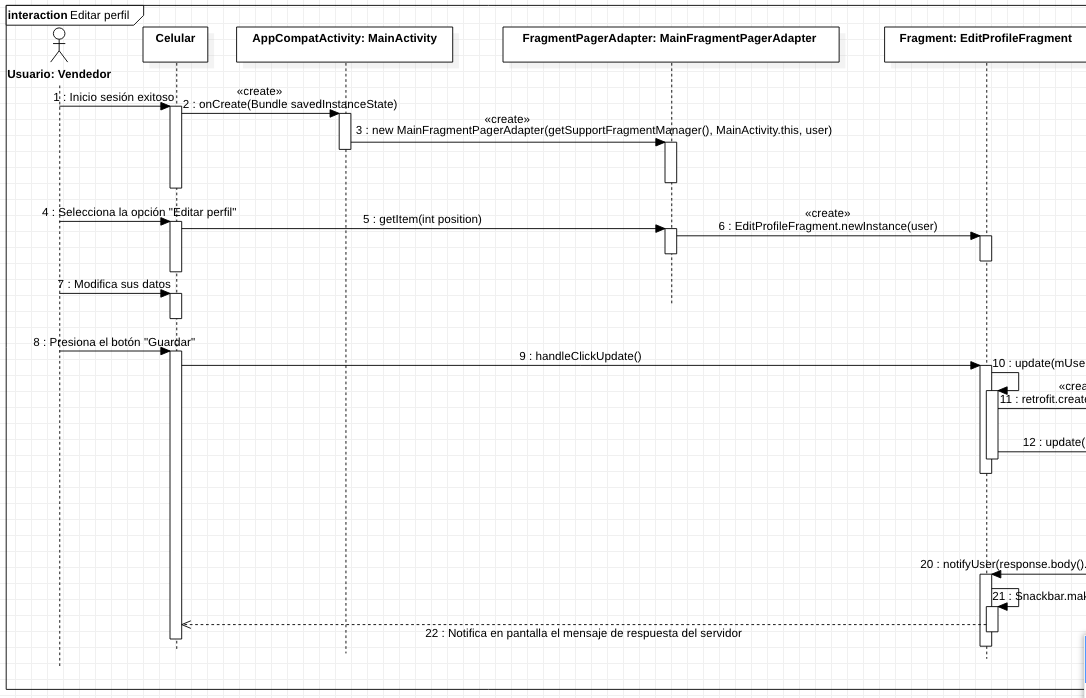
\includegraphics[width=1 \textwidth]{imagenes/adrian/vendedor/prototipo2/editar_perfil_1}
		\caption{Diagrama de secuencia para editar perfil de un vendedor (Parte 1).}
		\label{secuencia-AIPV2-perfilUno}
\end{figure}
\FloatBarrier

\FloatBarrier
\begin{figure}[htbp!]
		\centering
			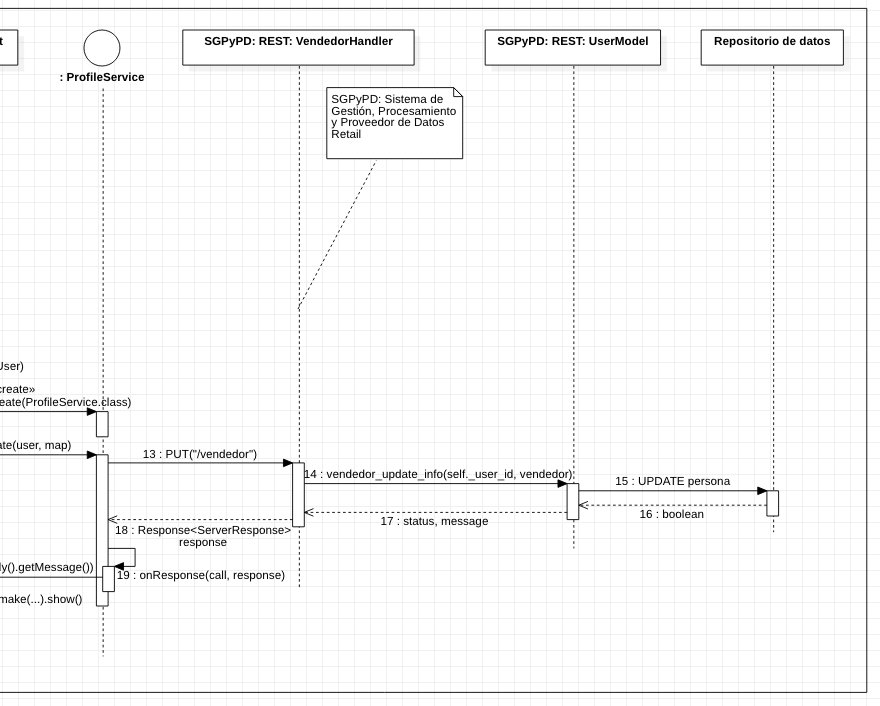
\includegraphics[width=1 \textwidth]{imagenes/adrian/vendedor/prototipo2/editar_perfil_2}
		\caption{Diagrama de secuencia para editar perfil de un vendedor (Parte 2).}
		\label{secuencia-AIPV2-perfilDos}
\end{figure}
\FloatBarrier

\title{\textbf{Ver clientes cercanos.}\\}

En la figura \ref{secuencia-AIPV2-cercanos} se muestra el diagrama de secuencia para ver clientes cercanos en la AIPV, es decir, mostrarle al usuario vendedor los usuarios que se han conectado previamente a un Beacon en el departamento que se encuentre. Para una mejor visualización el diagrama se ha dividido en 2 partes las cuales se muestran en las figuras \ref{secuencia-AIPV2-cercanosUno} y \ref{secuencia-AIPV2-cercanosDos} .

\FloatBarrier
\begin{figure}[htbp!]
		\centering
			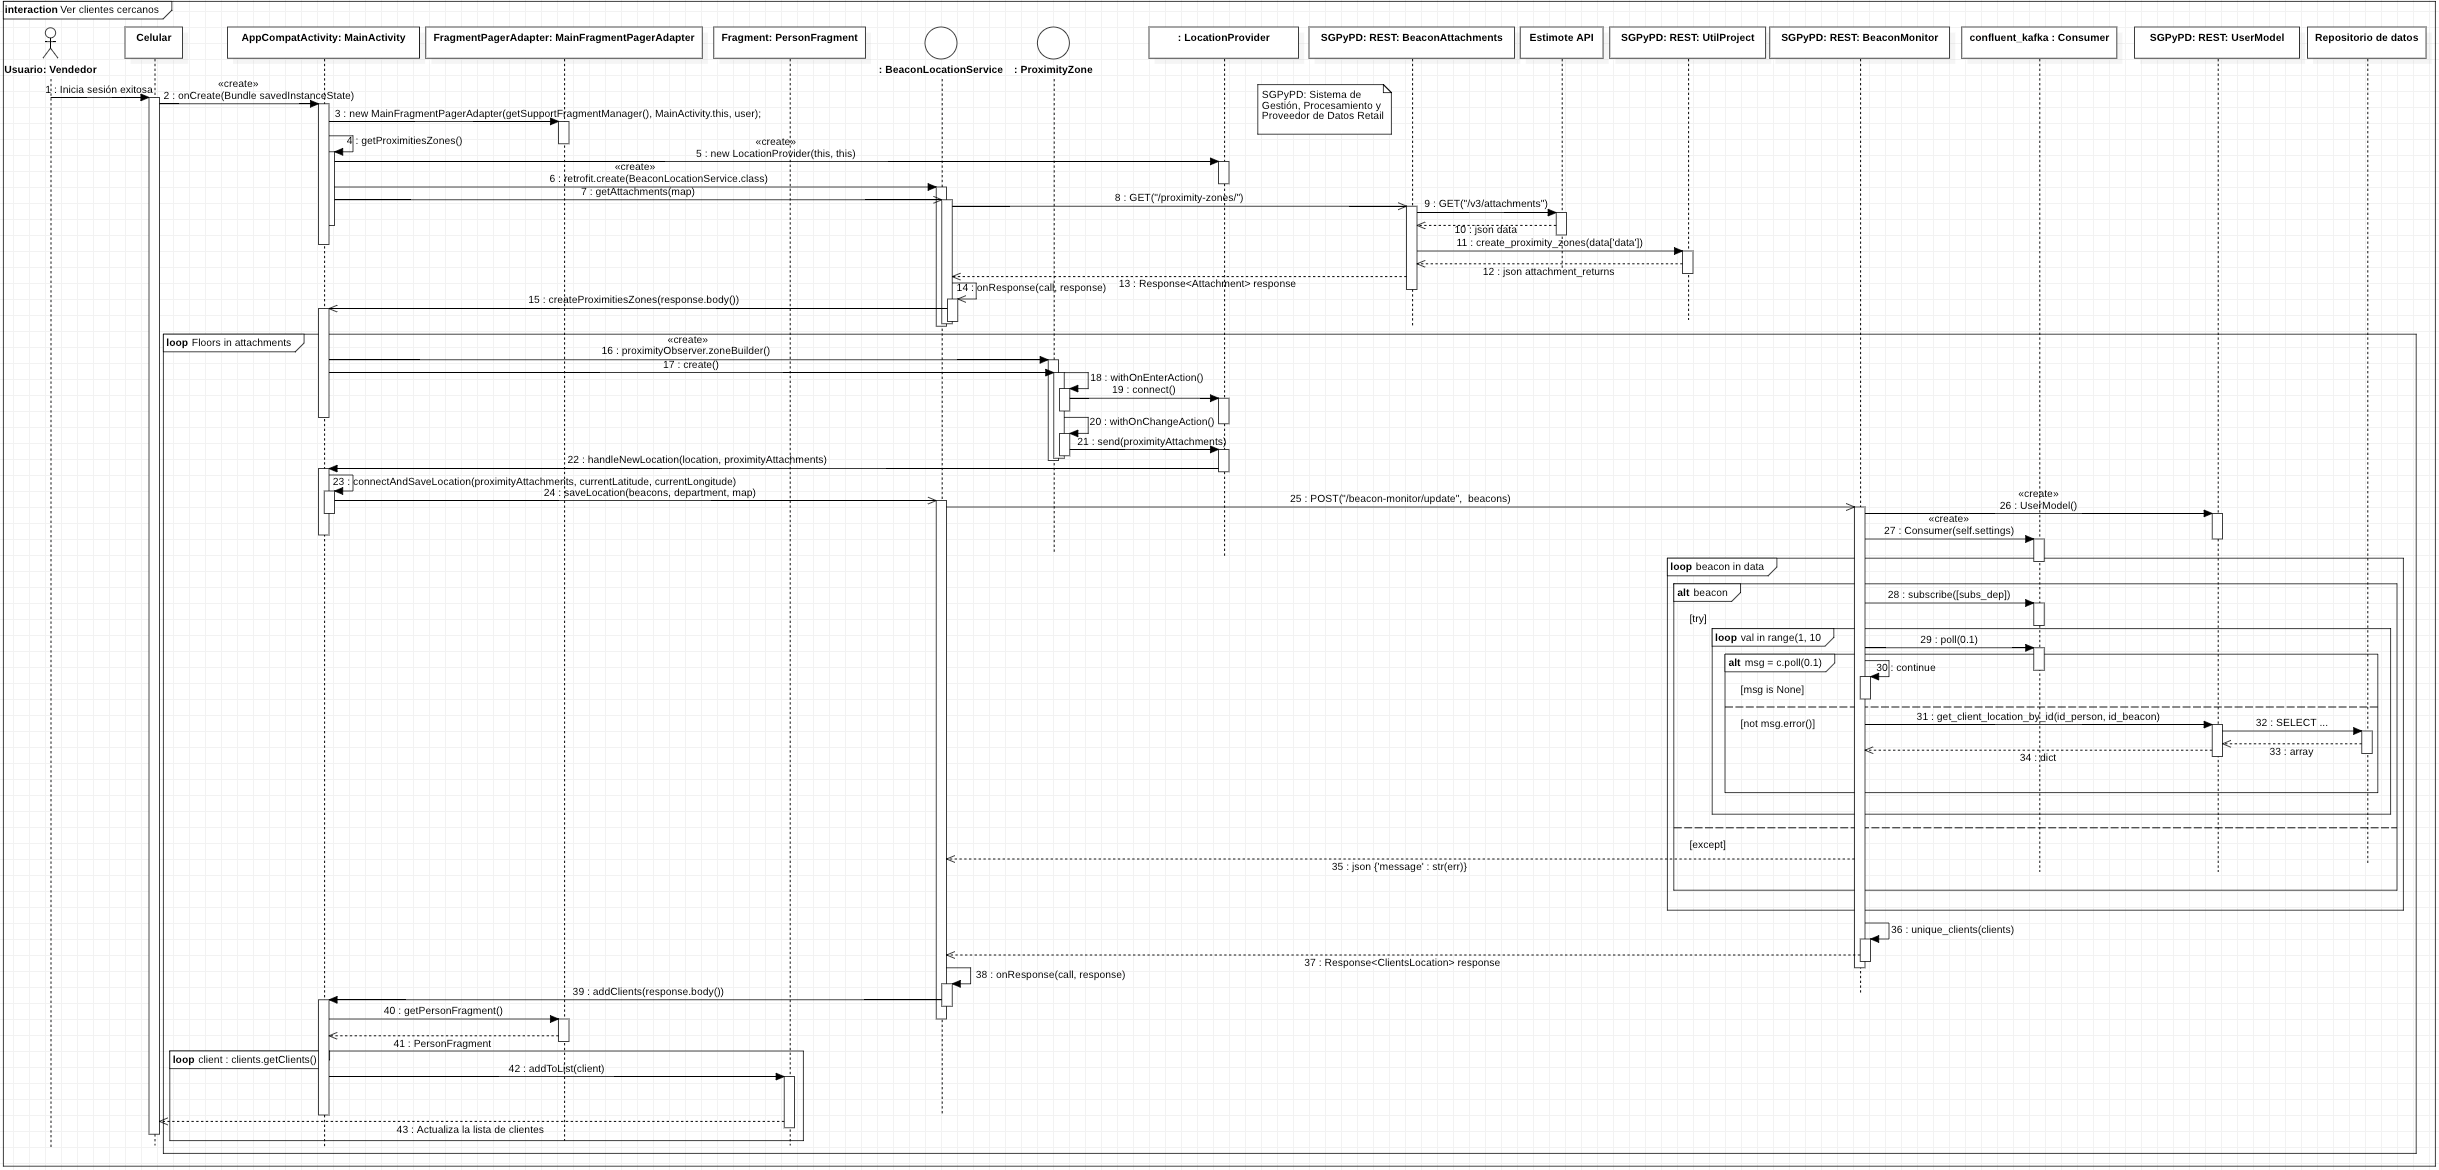
\includegraphics[width=1 \textwidth]{imagenes/adrian/vendedor/prototipo2/clientes_cercanos}
		\caption{Diagrama de secuencia para ver a los clientes cercanos en la aplicación.}
		\label{secuencia-AIPV2-cercanos}
\end{figure}
\FloatBarrier

\FloatBarrier
\begin{figure}[htbp!]
		\centering
			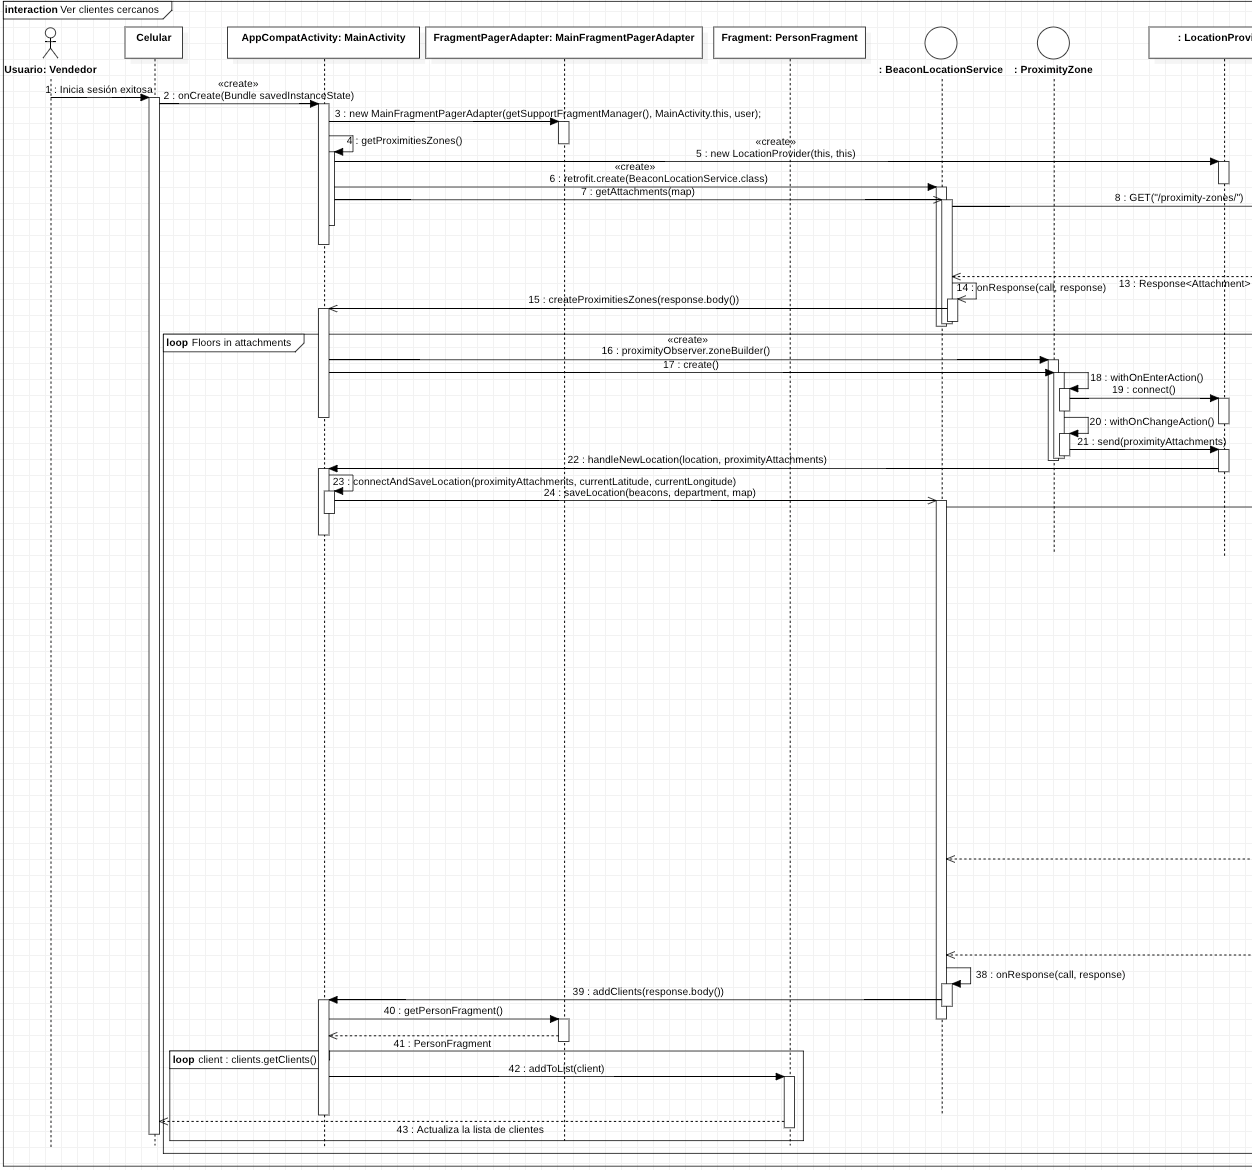
\includegraphics[width=1 \textwidth]{imagenes/adrian/vendedor/prototipo2/clientes_cercanos_1}
		\caption{Diagrama de secuencia para ver a los clientes cercanos en la aplicación (Parte 1).}
		\label{secuencia-AIPV2-cercanosUno}
\end{figure}
\FloatBarrier

\FloatBarrier
\begin{figure}[htbp!]
		\centering
			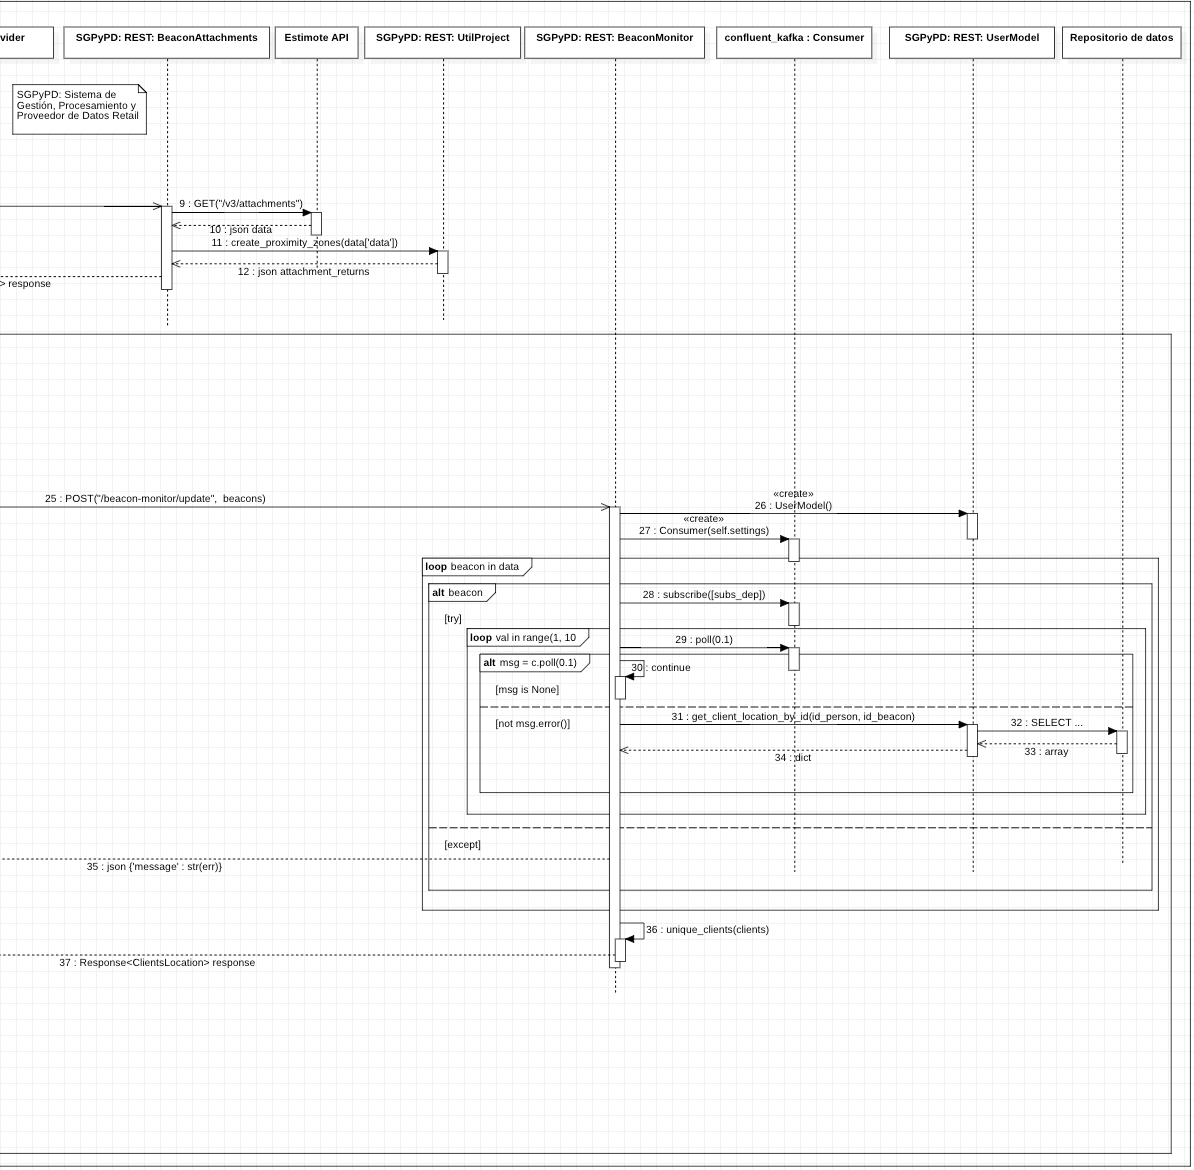
\includegraphics[width=1 \textwidth]{imagenes/adrian/vendedor/prototipo2/clientes_cercanos_2}
		\caption{Diagrama de secuencia para ver a los clientes cercanos en la aplicación (Parte 2).}
		\label{secuencia-AIPV2-cercanosDos}
\end{figure}
\FloatBarrier

%\paragraph{Flujo de navegación de la AIPV.} ~\\

%La siguiente figura \ref{navegacion-AIPV2} muestra como es el flujo de navegación de la aplicación para el prototipo 2.

%\FloatBarrier
%\begin{figure}[htbp!]
%		\centering
%			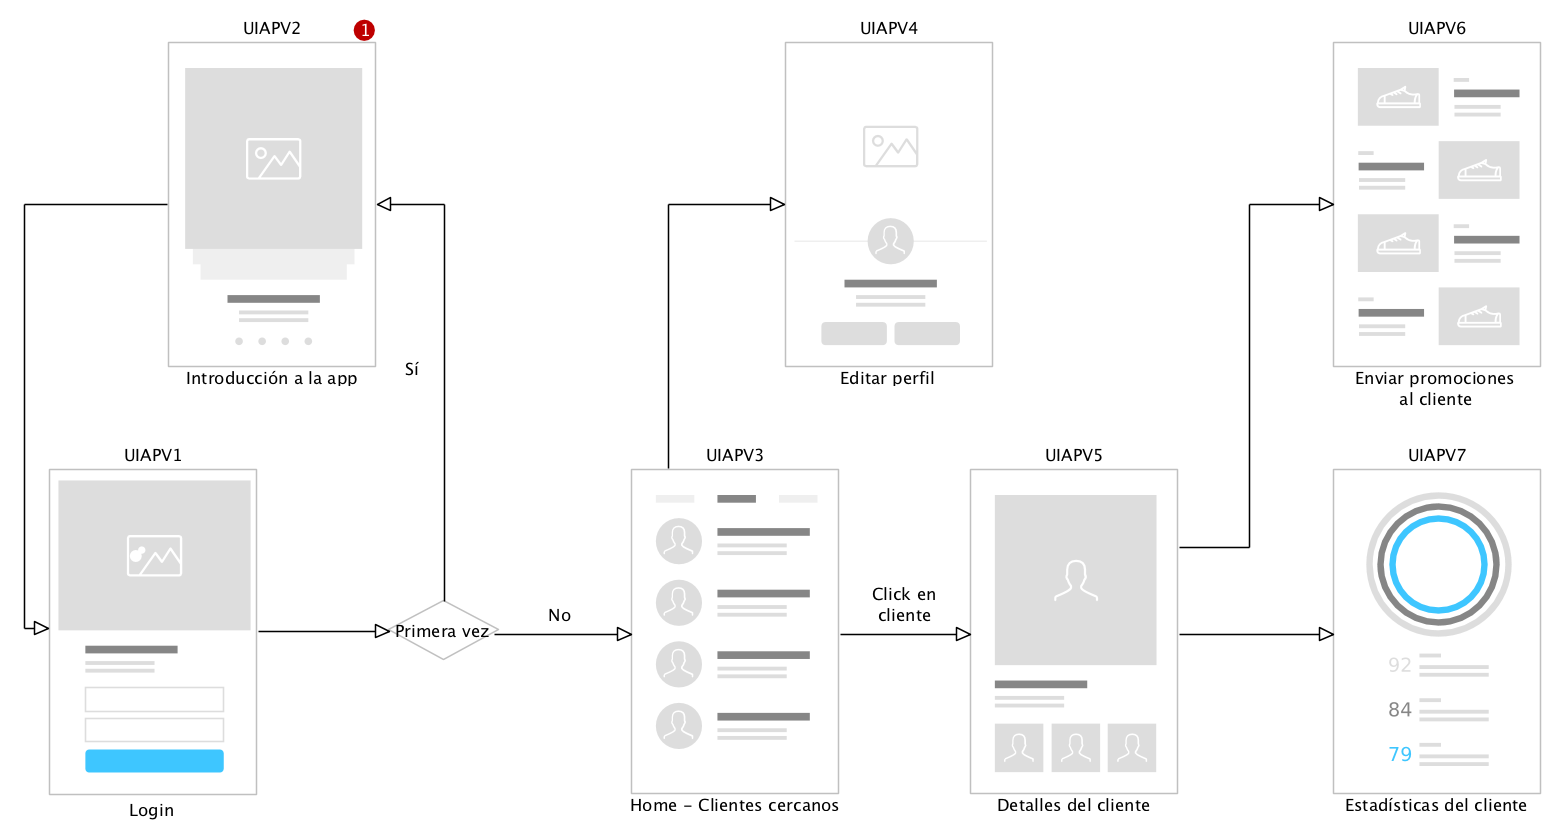
\includegraphics[width=1 \textwidth]{imagenes/adrian/vendedor/prototipo2/UIApp/0}
%		\caption{Flujo de navegación de la AIPV para el prototipo 2.}
%		\label{navegacion-AIPV2}
%\end{figure}

%\paragraph{Interfaces de usuario}

%\cfinput{appMovil/Vendedor/prototipo2/UI/UIAPV1}
%\cfinput{appMovil/Vendedor/prototipo2/UI/UIAPV2}
%\cfinput{appMovil/Vendedor/prototipo2/UI/UIAPV3}
%\cfinput{appMovil/Vendedor/prototipo2/UI/UIAPV4}
%\cfinput{appMovil/Vendedor/prototipo2/UI/UIAPV5}
%\cfinput{appMovil/Vendedor/prototipo2/UI/UIAPV6}
%\cfinput{appMovil/Vendedor/prototipo2/UI/UIAPV7}
%--------------------------------------------------
%\subsubsection{Pruebas}

